
 \begin{slide}{EXAFS: Extended X-ray Absorption Fine Structure}

 \begin{cenpage}{130mm}

   Far above the edge, the oscillations in $\mu(E)$ are sensitive to the
   distances and types of atoms neighboring the absorbing atom.  \vmm

  We define the EXAFS $\chi$ as the oscillations in $\mu(E)$:

   \[
     \mu(E) =   \mu_0(E) [1 + \chi(E)]
     \hspace{15mm} \chi(E) =   \frac{ {\mu(E) - \mu_0(E)}}{\Delta \mu_0(E_0)}
   \]

   We subtract off a smooth {\BlueEmph{``bare atom'' background}}
   $\mu_0(E)$, and divide by the {\BlueEmph{``edge step''}}
   $\Delta \mu_0(E_0)$ to get $\chi$, the EXAFS oscillations:

   \begin{columns}[T]
     \begin{column}{65mm}
       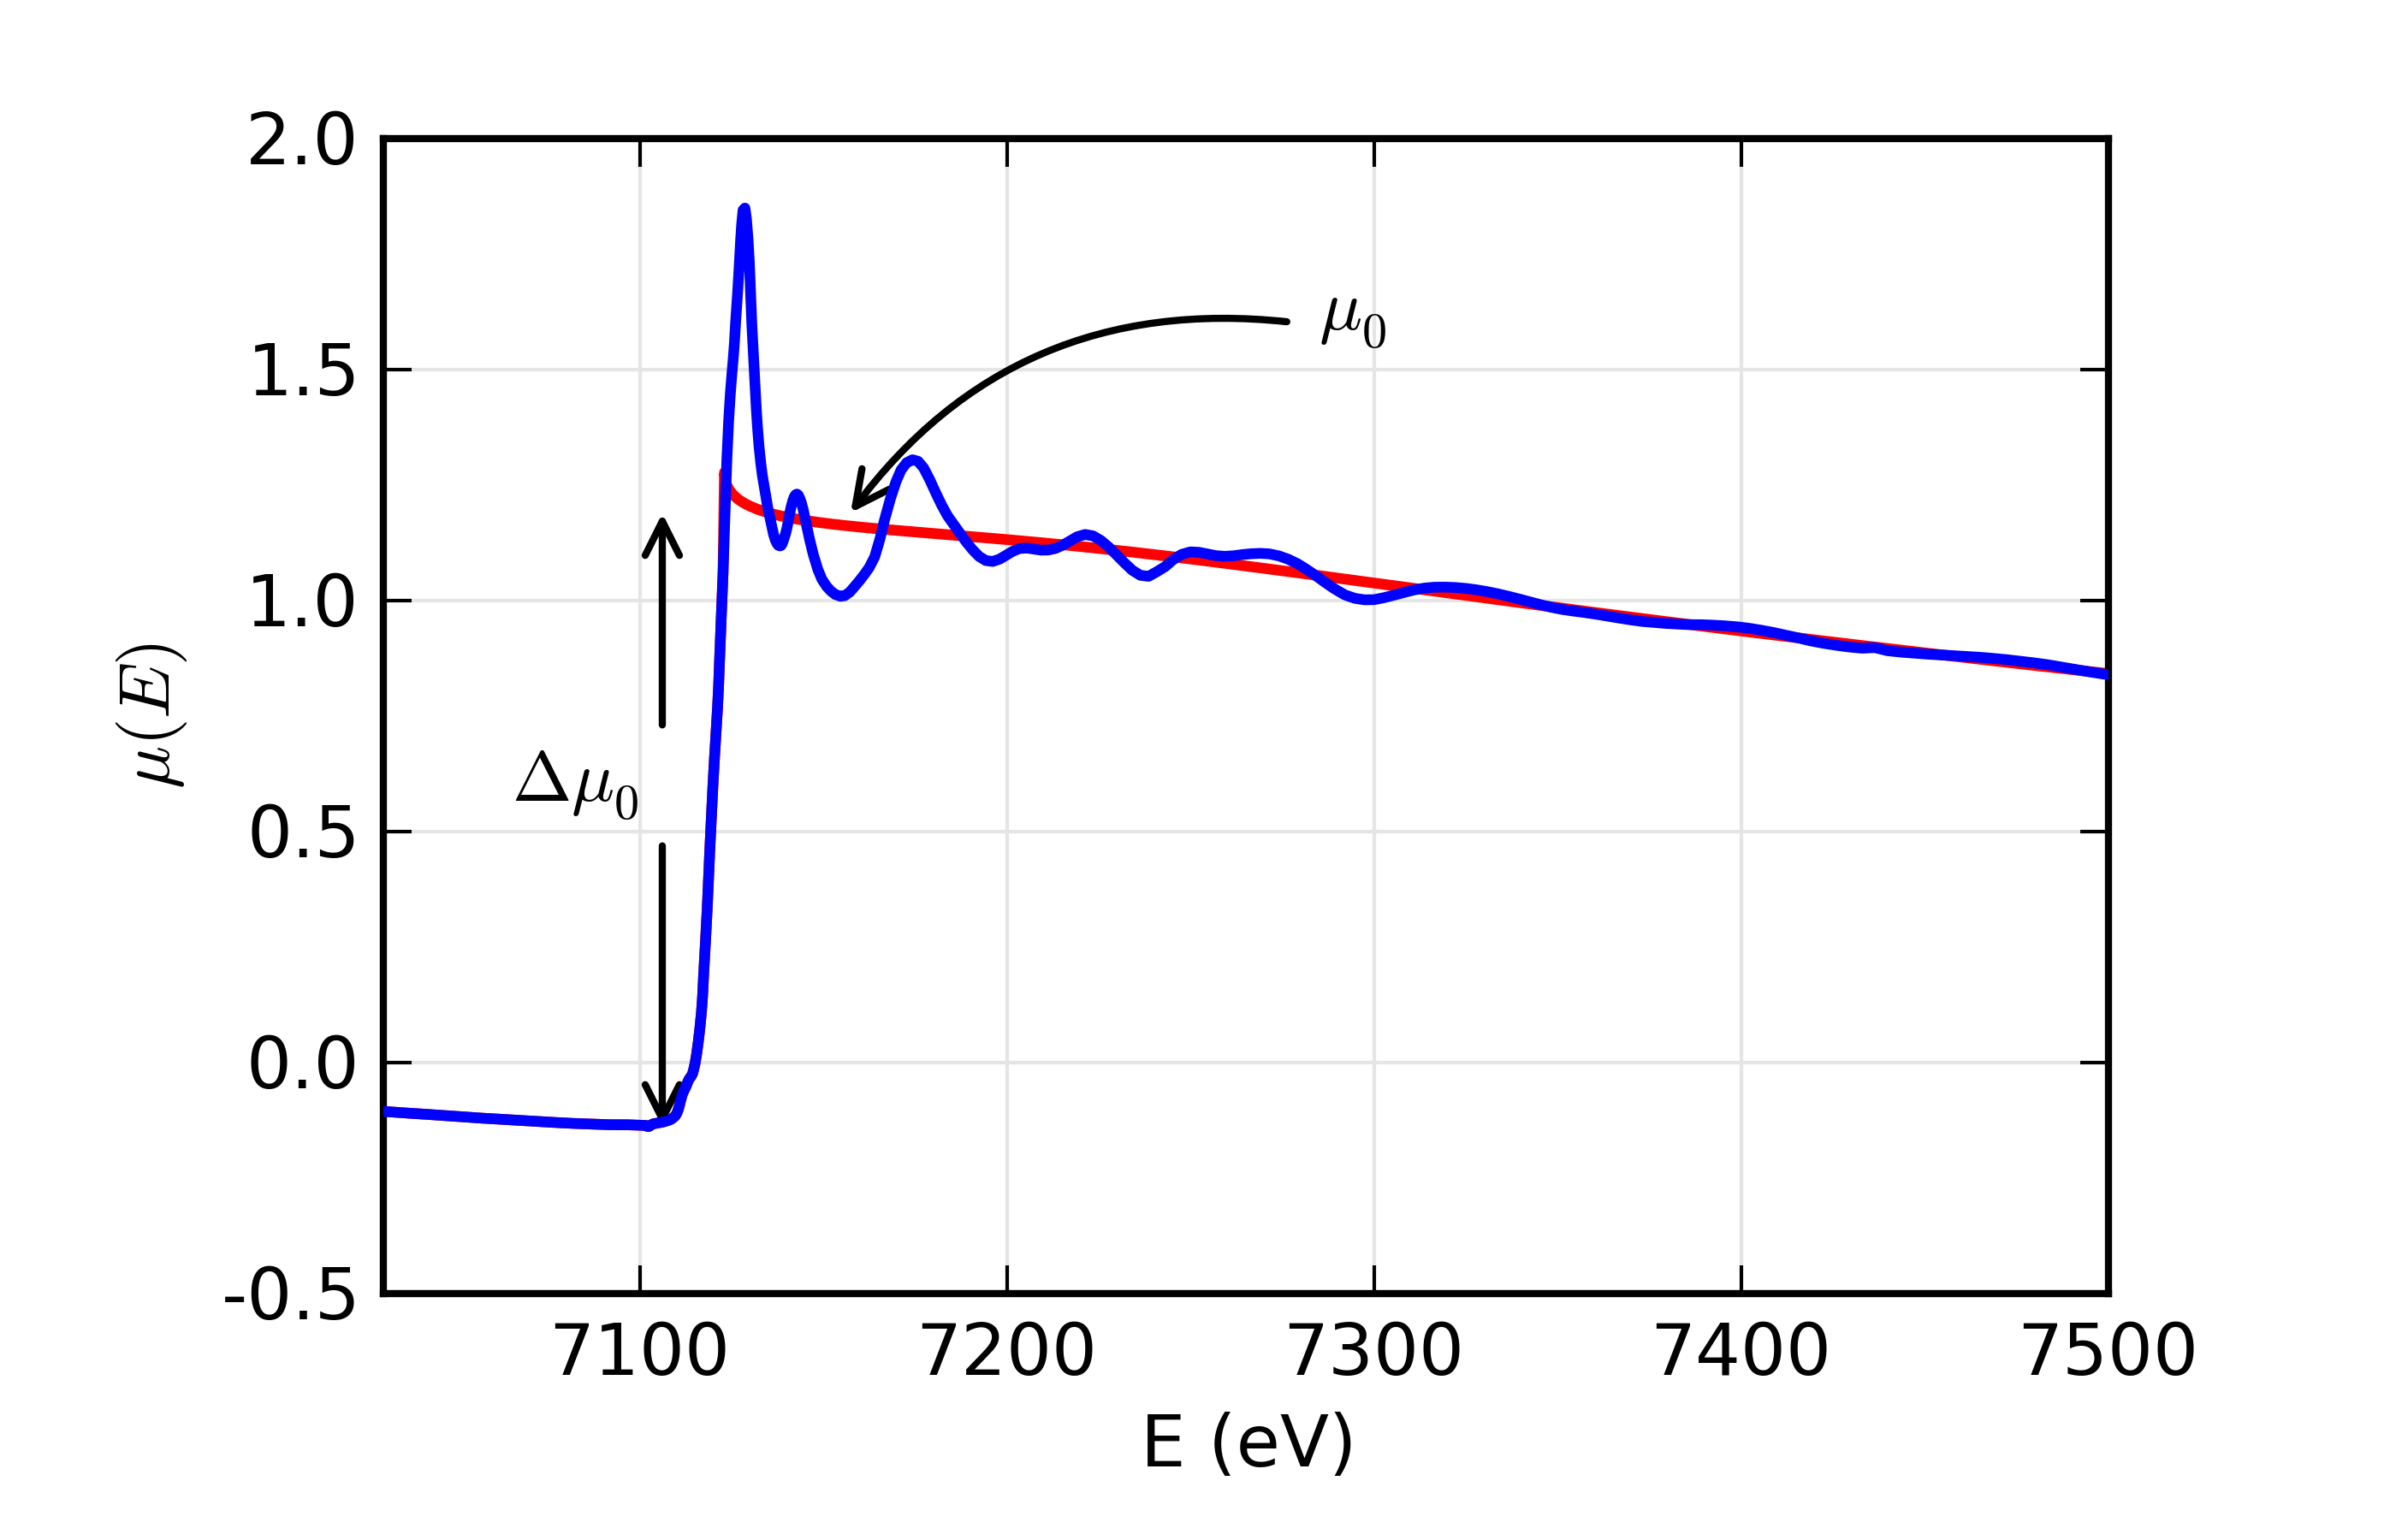
\includegraphics[width=58mm]{figs/rimg/mu_with_mu0}

       \hspace{10mm} $\mu(E)$ and $\mu_0(E)$ for FeO       
     \end{column}
     \begin{column}{65mm}
       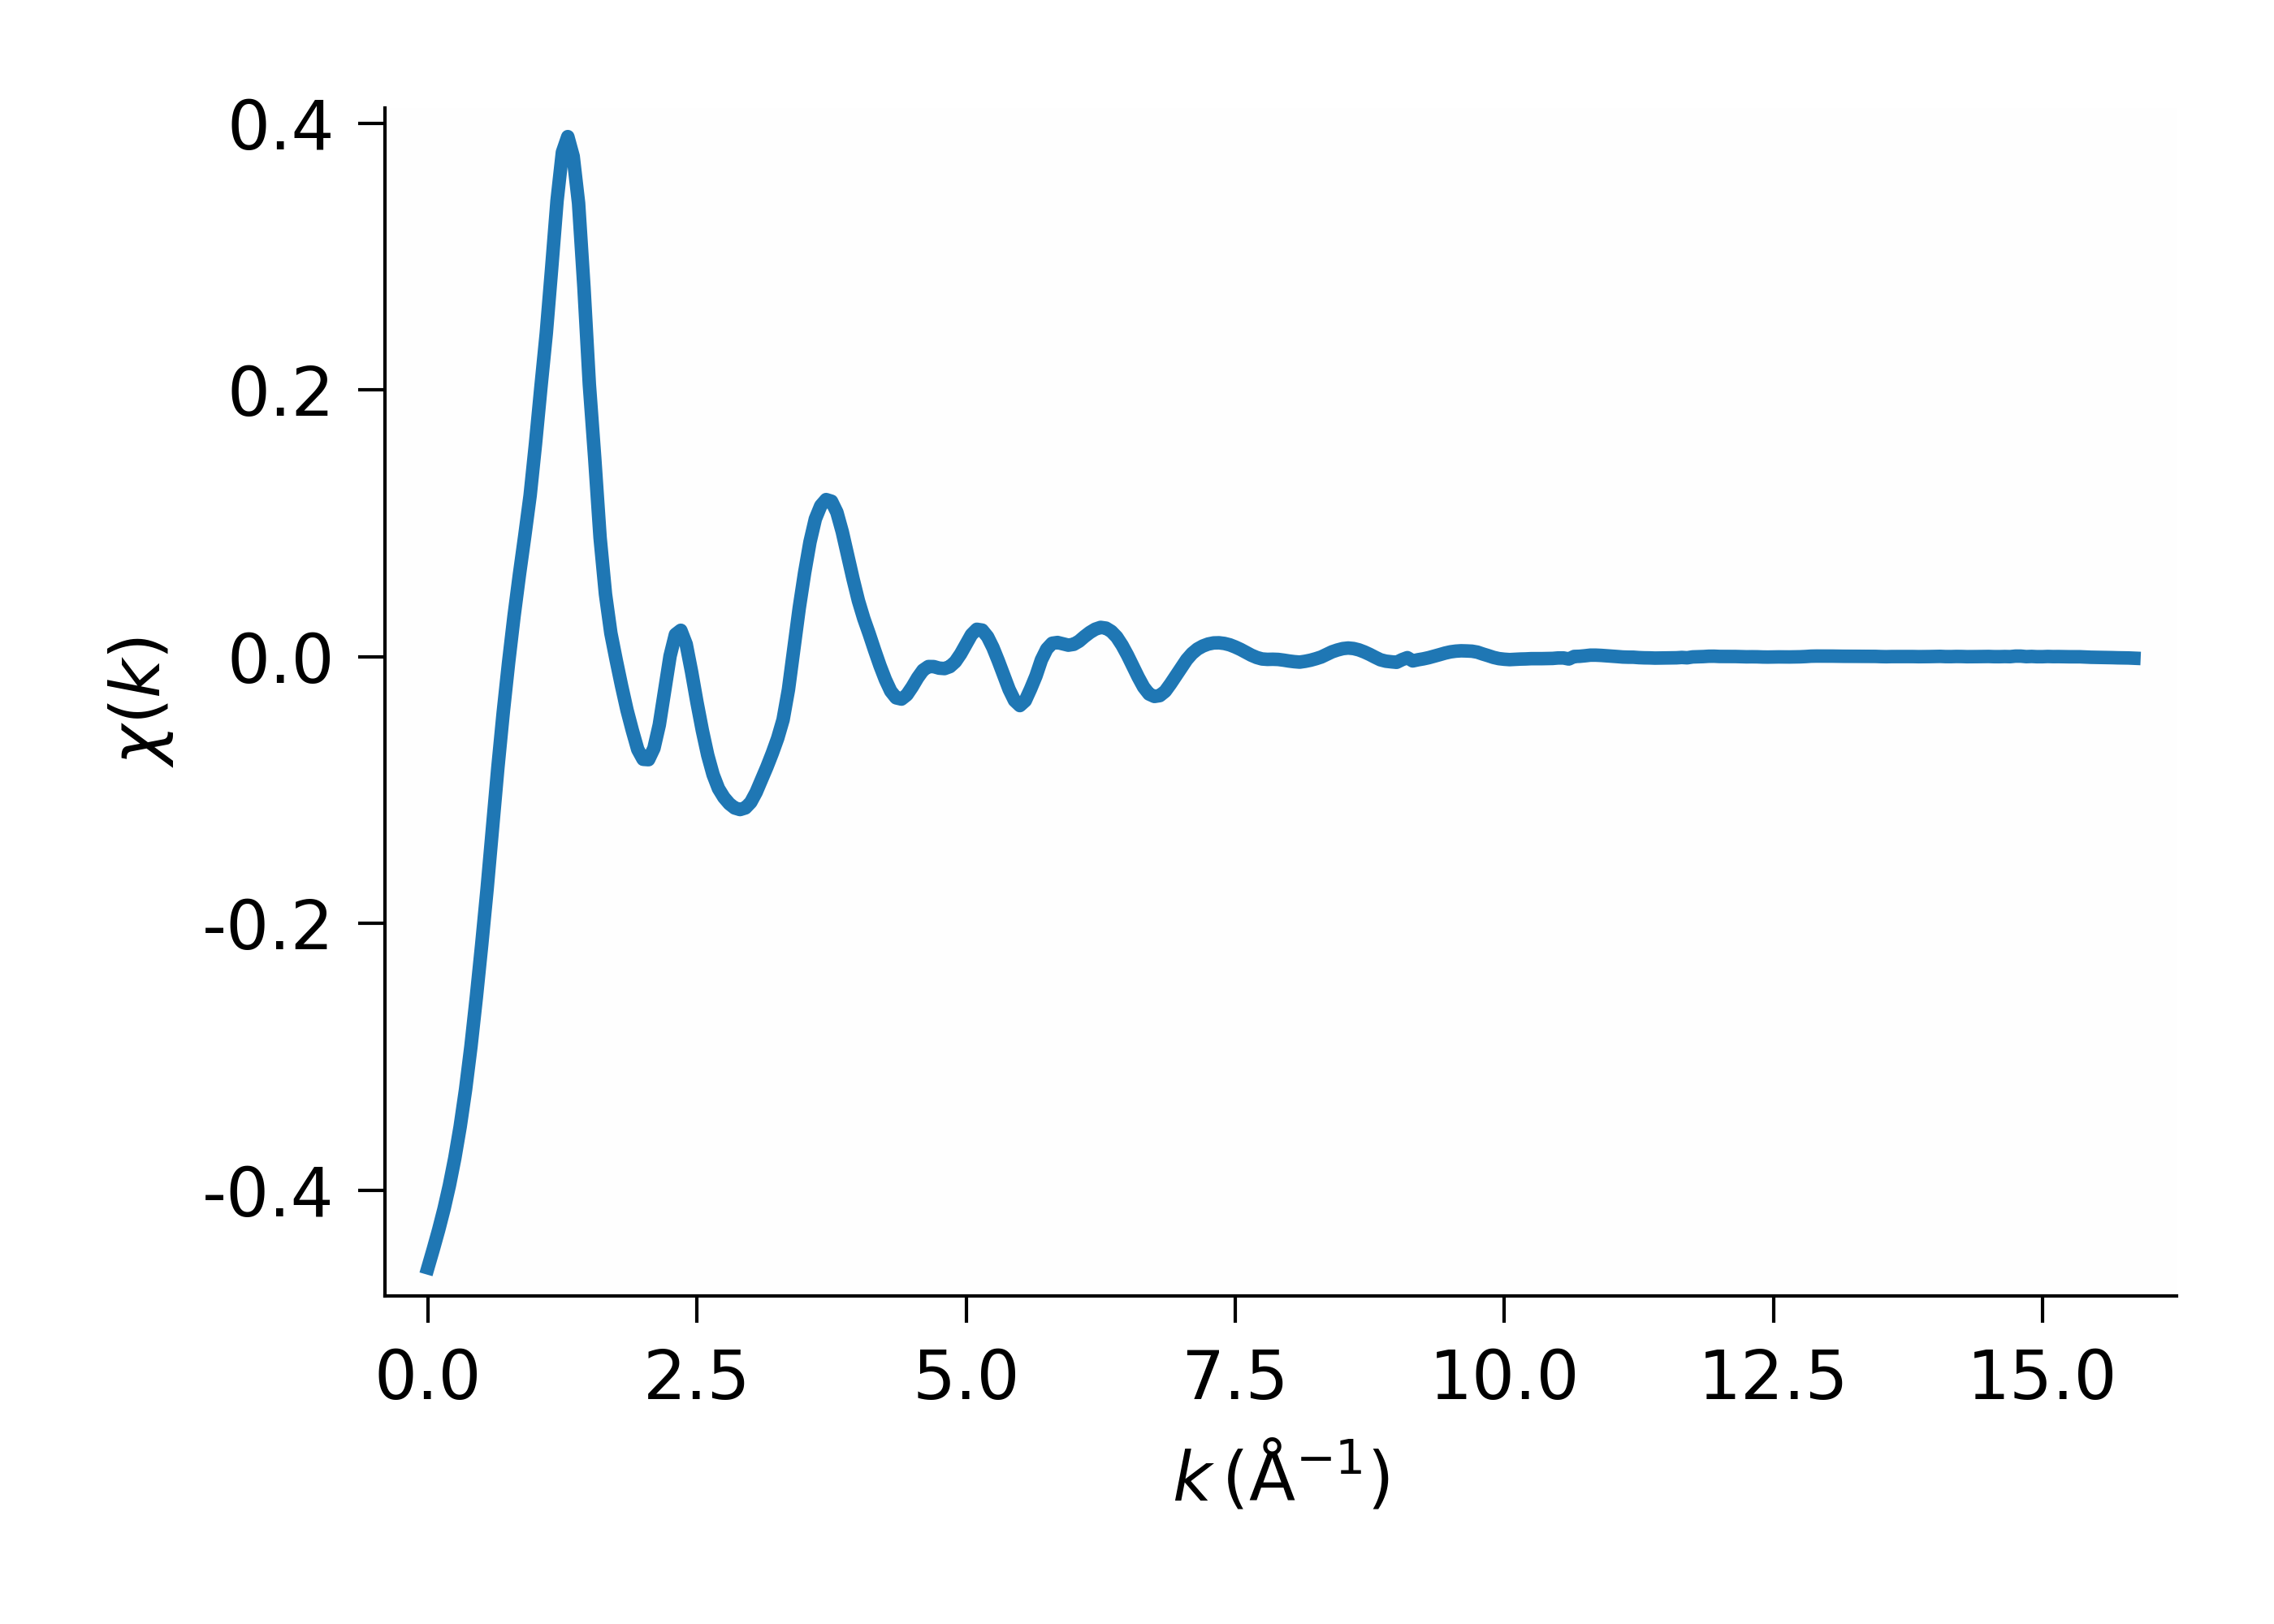
\includegraphics[width=58mm]{figs/rimg/chie}
       \hspace{10mm} $\chi(E)$ for FeO
     \end{column}     
   \end{columns}

 \end{cenpage}

 \vfill
\end{slide}

